%% LyX 2.1.3 created this file.  For more info, see http://www.lyx.org/.
%% Do not edit unless you really know what you are doing.

\documentclass[english]{beamer}
\usepackage[T1]{fontenc}
\usepackage[latin9]{inputenc}
\usepackage{amsmath}

\makeatletter
%%%%%%%%%%%%%%%%%%%%%%%%%%%%%% Textclass specific LaTeX commands.
 % this default might be overridden by plain title style
 \newcommand\makebeamertitle{\frame{\maketitle}}%
 % (ERT) argument for the TOC
 \AtBeginDocument{%
   \let\origtableofcontents=\tableofcontents
   \def\tableofcontents{\@ifnextchar[{\origtableofcontents}{\gobbletableofcontents}}
   \def\gobbletableofcontents#1{\origtableofcontents}
 }

%%%%%%%%%%%%%%%%%%%%%%%%%%%%%% User specified LaTeX commands.
\usetheme{Rochester}
\usecolortheme{beaver}

\usenavigationsymbolstemplate{}
\setbeamercolor{structure}{fg=darkred}
\setbeamercolor{block body}{bg=gray!10!white}

\makeatother

\usepackage{babel}
\begin{document}
\title{Accelerating your Python Code}
\subtitle{With PyCuda and GMMs}

\author{Varun Nayyar}


\date{27/07/18}
\makebeamertitle

\begin{frame}[t]\frametitle{Outline}
Me = Math Major + Script Kiddy (Manage Expectations please)
 
\begin{block}{What to Expect}
  \begin{itemize}
    \item Some Math
    \item Iterative Process I went through
    \item Thinking with CUDA
    \item How to use PyCUDA to avoid complicated work
  \end{itemize}

\end{block}

\begin{alertblock}{What not to Expect}
  \begin{itemize}
    \item How PyCUDA does it's magic
    \item Advanced CUDA (or even Intermediate)
  \end{itemize}
\end{alertblock}


\end{frame}



\begin{frame}[t]\frametitle{Gaussian Mixture Models d=1, K=2}
    \begin{center}
        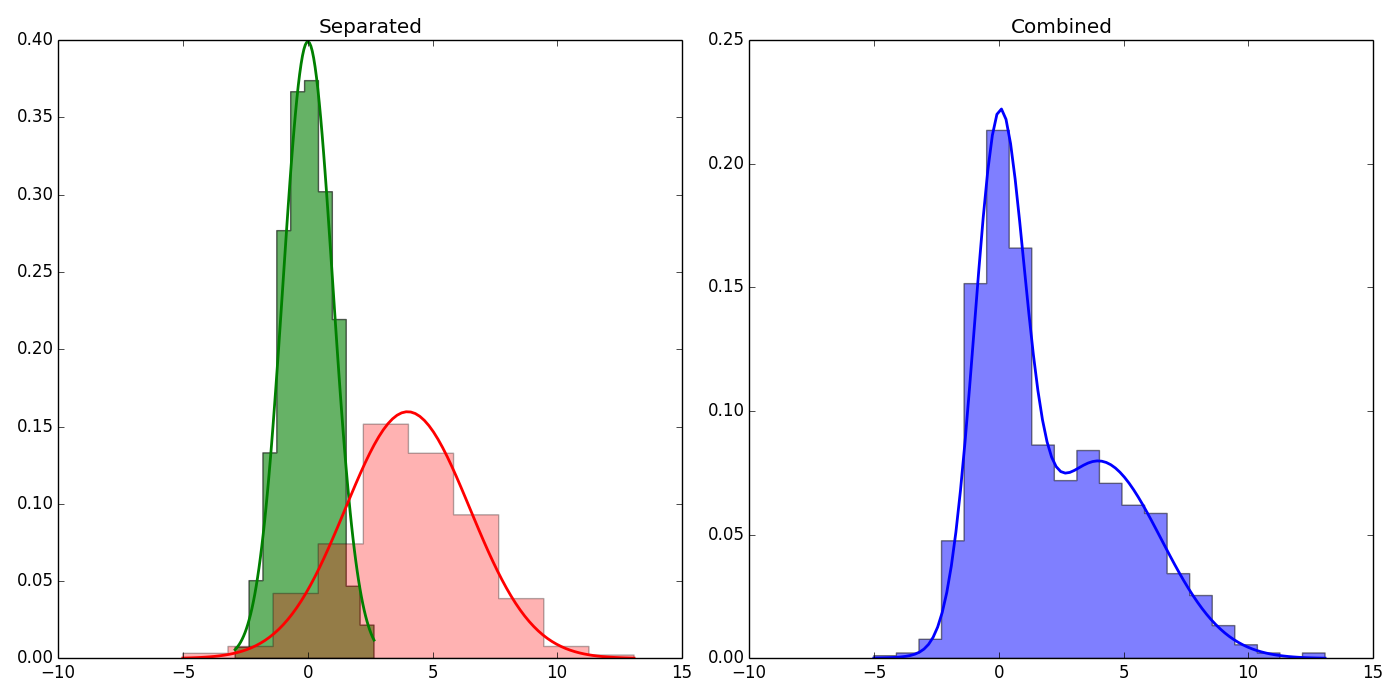
\includegraphics[width=10cm]{img/Combined.png}
    \end{center}
    
\end{frame}


\begin{frame}[t]\frametitle{Gaussian Mixture Models (GMMs)}

\begin{block}{Mathematical Notation}

Gaussian Mixture Models are a class of models that assume the data
points are generated by a finite number of gaussian (or normal) distributions
\begin{align*}
f(\mathbf{x}|\boldsymbol{\pi},\boldsymbol{\mu},\boldsymbol{\Sigma})= & \sum_{k=1}^{K}\pi_{k}\mathcal{N}(\mathbf{x}|\mu_{k},\Sigma_{k}) \\
l(\mu,\Sigma,\mathbf{x})  = &\sum_{i=1}^{N}\ln\left(\sum_{k=1}^{K}\pi_{k}\mathcal{N}(x_{i}|\mu_{k},\Sigma_{k})\right)\label{eq:LogLikelihood}
\end{align*}
with $K$ mixtures and the weights $\pi_{k}$ giving the prior probability
of mixture component $k$ (and sum to 1).
\end{block}

\end{frame}


\begin{frame}[t]\frametitle{Doing it Live}

\begin{columns}

  \column{0.5\textwidth}
  This can't 


  \column{0.5\textwidth}
    \begin{center}
        
\includegraphics[height=6cm]{img/doingitlive.jpg}
    \end{center}

\end{columns}

\end{frame}

\begin{frame}[t]\frametitle{Need for speed}
\begin{itemize}
    \item GMM likelihood formula doesn't decompose into a mathematically simpler form
    \item Number of flops are of the order of O(NKd), in my case, N = 100,000, K = 8, d = 13. 
    \item I needed to evaluate the likelihood 100,000 times for a fixed dataset while the parameters were varied.
\end{itemize}        
\end{frame}








\end{document}

